\documentclass[11pt]{jsarticle}

\usepackage[top=30mm, bottom=36mm, left=28mm, right=28mm]{geometry}
\usepackage[dvipdfmx]{graphicx}

\usepackage{mytitle}

\title{1. FIFO IP Coreとは}
\author{201720690 小松 弘人}
\date{2017/06/12}

\makeatletter
\def\mojiparline#1{
    \newcounter{mpl}
    \setcounter{mpl}{#1}
    \@tempdima=\linewidth
    \advance\@tempdima by-\value{mpl}zw
    \addtocounter{mpl}{-1}
    \divide\@tempdima by \value{mpl}
    \advance\kanjiskip by\@tempdima
    \advance\parindent by\@tempdima
}
\makeatother
\def\linesparpage#1{
    \baselineskip=\textheight
    \divide\baselineskip by #1
}

\begin{document}
\maketitle
\subsection*{First-In First-Out (FIFO)}

First-In First-Out (FIFO) は先入れ先出しと訳される。
これは、キューの動作を表すものであり、入力された順にデータが出力される
(図\ref{img:queue})。
Vivadoでは、FIFO Generatorを用いてこのメモリキューを利用できる。

\begin{figure}[ht]
	\centering
	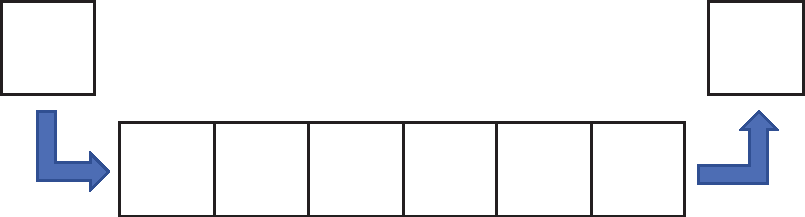
\includegraphics[width=0.6\linewidth]{img/queue.pdf}
	\caption{First-In First-Out (Queue)}
	\label{img:queue}
\end{figure}

\vspace{-0.3cm}

FIFO IP Coreの主な入出力には、次のようなものがある (図\ref{img:fifo_ip})。
\begin{figure}[ht]
	\centering
	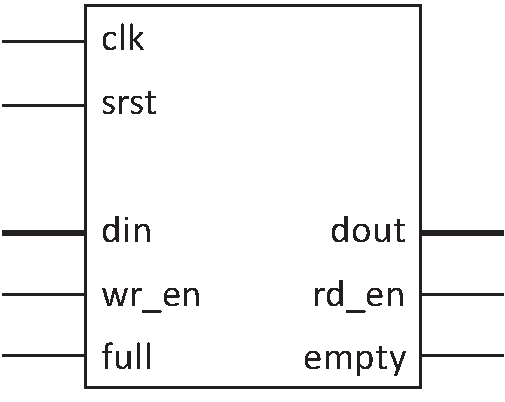
\includegraphics[width=4cm]{img/fifo_ip.pdf}
	\caption{FIFO IP Core}
	\label{img:fifo_ip}
\end{figure}

\vspace{-0.3cm}

主な入出力は以下の通り。
詳細は、FIFO Generatorのドキュメント (PG057) を参照。
\begin{itemize}
	\item
		clk:
		クロック信号。
	\item
		srst:
		同期リセット信号 (Synchronous ReSeT)。
		srst=1のとき、クロックの立ち上がりでFIFO IP Coreをリセットする。
	\item
		din:
		データ入力信号。
	\item
		wr\_en:
		書き込みイネーブル信号。
		wr\_en=1のとき、クロックの立ち上がりでデータを取り込む。
	\item
		full:
		FIFOにこれ以上データが入らないとき、full=1。
	\item
		dout:
		データ出力信号。
	\item
		rd\_en:
		読み出しイネーブル信号。
		rd\_en=1のとき、クロックの立ち上がりで出力値を変更する
		(読み出されたと判断する)。
	\item
		empty:
		FIFOにデータが入っていないとき、empty=1。
		FIFOの動作モード (後述) によって、
		値が変化するタイミングが異なるので注意。
\end{itemize}

\subsection*{FIFOの動作モード}
FIFO IP Coreには、StandardモードとFirst Word Fall Through (FWFT)モードの
2つの動作モードがある。
これらのモードの違いは、データ出力信号と
empty信号の値が変わるタイミングである。

Standardモードでは、empty=1になった次のクロックからデータが出力される。
一方、FWFTモードでは、empty=1になったクロックから、データが出力される。
つまり、FWFTモードで動作するFIFOの方がFIFO同士を連結させやすい。

詳しくは、2つのFIFOのシミュレーション波形
(図\ref{img:cmp_fifo}) を確認のこと。

\subsection*{FIFOのシミュレーション}
FIFOの動作をシミュレータで確認する。
ここでは、StandardモードとFWFTモードのFIFOのシミュレーションを行った。
動作モードによる入出力信号の変化の違いに注目。

\begin{figure}[ht]
	\centering
	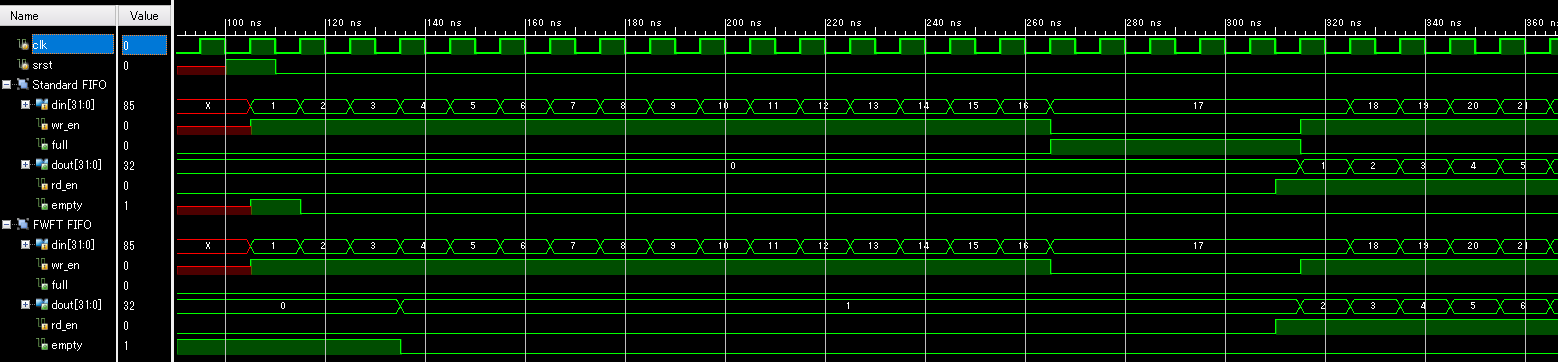
\includegraphics[width=\linewidth]{img/cmp_fifo.PNG}
	\caption{シミュレーション波形}
	\label{img:cmp_fifo}
\end{figure}

\vspace{-1cm}

\subsection*{FIFOの連結}
複数のFIFOを連結し、1つのFIFOとして動作するブロックを作ることができる
(図\ref{img:fifo_join})。
これを応用し、FIFO間に計算用回路を置くことで
画像フィルタなどが計算できる。
入出力信号のタイミングの関係から、前段のFIFOはFWFTモードのものを用いる。
詳細は``2013.3 FIFO Generator v11.0 - 小型FIFOを複数使用した
深さおよび幅の値が大きな FIFO の作成'' (AR\# 58928) を参照のこと。

\begin{figure}[ht]
	\centering
	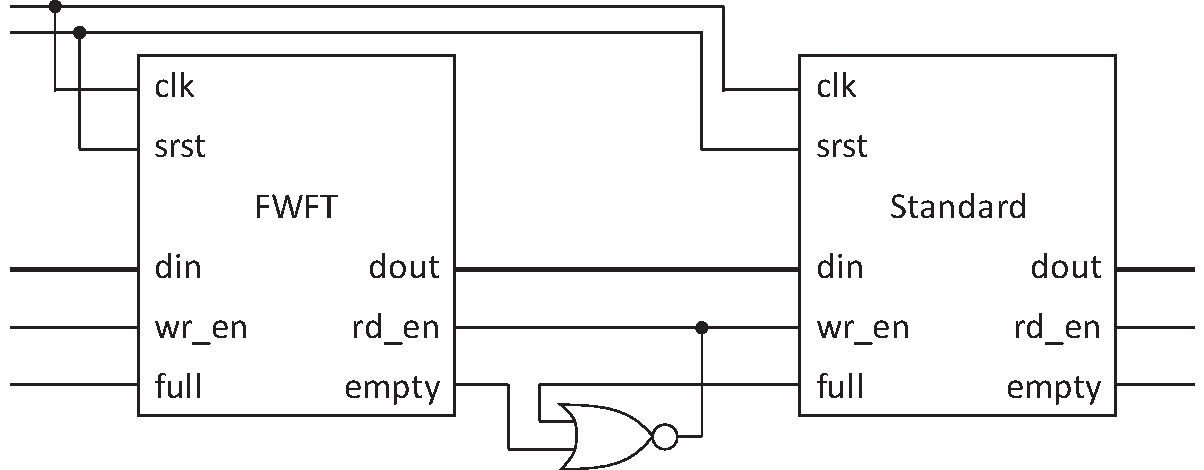
\includegraphics[width=0.5\linewidth]{img/fifo_join.pdf}
	\caption{FIFOの連結}
	\label{img:fifo_join}
\end{figure}

\end{document}
